Во избежание повторений продемонстрирую как выглядит моё сообщение, закодированное с помощью потенциального метода NRZ:
Для определения верхней границы частот необходимо найти наиболее высокочастотную составляющую спектра в передаваемом сообщении, которая в NRZ образуется при передаче чередующихся значений 0 и 1, при этом период гармонического сигнала (синусоиды), используемого для передачи прямоугольных сигналов 0 и 1, будет равен удвоенной длительности битового интервала $\tau: T = 2\tau$, где $\tau$ определяется как величина, образная значению пропускной способности канала $C: \tau = \frac{1}{C}$. Отсюда верхняя граница частот будет равна \[f_{\text{в}} = \frac{1}{T} = \frac{C}{2}\]

То есть, при пропускной способности канала связи $C = 10 \, \text{Мбит/с}$ частота основной гармоники равна $f_{\text{в}} = \frac{10 \cdot 10^3}{2} = 5 \, \text{МГц}$, а битовый интервал $\tau = 100 \, \text{нс}$.

В общем случае, при кодировании любого сообщения с помощью метода NRZ наибольшая (верхняя) частота достигается при передаче чередующихся значений 0 и 1, а наименьшая (нижняя) - при передаче длинных (в пределе - бесконечных) последовательностей нулей и единиц, что делает нижнюю границу частот близкой и в пределе равной нулю: $f_{\text{н}} = 0$. Следовательно, в предельном случае спектр: $S = f_{\text{в}} - f_{\text{н}} = f_{\text{в}} = \frac{C}{2}$.

С другой стороны, при передаче конкретного сообщения нижняя частота всегда больше нуля и зависит от максимальной длины последовательностей нулей или единиц. В этом случае для расчёта нижней границы чапстот необходимо в коде передаваемого сообщения найти \textit{наиболее длинную последовательность 1 или 0}. В исходном сообщении, закодированном по методу NRZ, представленному на рисунке 1, низкочастотная составляющая образуется при передаче 6 последовательных нулей. Период синусоидального сигнала при передаче таких последовательностей равен 12 битовым интервалам и нижняя граница частот соответственно будет равна: $f_{\text{н}} = \frac{1}{12\tau} = \frac{C}{12}$. Тогда \textbf{спектр} при передаче данного сообщения кодом NRZ равен
\[
	S =  f_{\text{в}} - f_{\text{н}} = \frac{C}{2} - \frac{C}{12} = \frac{5C}{12} = 4.167 \, \text{МГц}
\]

Среднее значение частоты передаваемого сообщения находится в интервале $(f_{\text{н}};f_{\text{в}})$ и показывает, какие частоты (низкие или высокие) превалируют в спектре передаваемого сигнала.

Для оценки среднего значения частоты передаваемого сообщения можно для каждого битового интервала определить соответствующую частоту сигнала, просуммировать их и разделить на количество битовых интервалов. В нашем случае: частота основной гармоники $f_0 = \frac{C}{2}$ соответствует трём битовым интервалам, частота вдвое меньшая, т.е. $\frac{f_0}{2}$, соответствует также трём битовым интервалам, частота $\frac{f_0}{3}$ - четырём битовым интервалам, $\frac{f_0}{5}$ - одному битовому интервалу, и $\frac{f_0}{6}$ - одному битовому интервалу.

Тогда средняя частота рассматриваемого сообщения
\[
	f_{\text{ср}} = \left(3f_0+3\frac{f_0}{2}+4\frac{f_0}{3}+\frac{f_0}{5}+\frac{f_0}{6}\right)/ 12 = \frac{31f_0}{60} = \frac{31 \cdot 5}{60} \approx 2.583 \, \text{МГц}
\]

Поскольку середине спектра рассматриваемого сообщения соответствует частота
\[
	f_{1/2} = (f_{\text{н}} + f_{\text{в}}) /2 = \frac{\frac{C}{2} + \frac{C}{12}}{2} = \frac{7C}{24} = 2.917 \, \text{МГц}
\]
Можно констатировать, что в спектре сигнала \textit{незначительно превалируют низкие частоты}: $f_{\text{ср}} < f_{1/2}$.

Для качественной передачи двоичных сигналов по реальному каналу связи и возможности их распознавания на приёмной стороне с минимальным количеством ошибок, желательно на передающей стороне формировать сигналы, приближающиеся к прямоугольной форме. Однако, спектр таких сигналов оказывается слишком большим. Можно показать, что для качественного распознавания сигнала на приемной стороне при передаче чередующихся значений 0 и 1 достаточно сформировать сигнал, содержащий первые 4 гармоники (поскольку более высокочастотные гармоники оказывают незначительное влияние на результирующий сигнал) с частотами $f_0=\frac{C}{2}, f_1=3f_0, f_2=5f_0, f_3=7f_0$. В этом случае верхняя граница частот $f_{\text{в}}=7f_0$, а ширина спектра сигнала при передаче рассматриваемого сообщения соответственно будет равна $S = f_{\text{в}} - f_{\text{н}} = 7f_0-f_0/6=41f_0/6=34.167 \, \text{МГц}$.

Итак, при пропускной способности канала связи $C = 10 \, \text{Мбит/с}$ верхняя и нижняя границы частот в передаваемом сообщении равны соответственно $f_{\text{в}} = 5 \, \text{МГц}$ и $f_{\text{н}} = 0.833 \, \text{МГц}$, спектр сигнала $S = 4.167 \, \text{МГц}$, среднее значение частоты в спектре передаваемого сигнала $f_{\text{ср}} = 2.583 \, \text{МГц}$, полоса пропускания, необходимая для качественной передачи данного сообщения $F=35 \, \text{МГц}$.


Так должен выглядеть полученный сигнал при отсутствии ошибок.

\subsection{NRZ}

Для потенциального метода кодирования NRZ определим минимальную требуемую полосу пропускания \textit{идеального канала связи} для качественной передачи сообщения:
\begin{enumerate}
	\item Отсутствуют шумы и помехи
	\item Принимающие и передающие узлы абсолютно синхронизированны
	\item Сигналы не затухают $\Rightarrow$ не нужно устанавливать уровни граничного напряжения
\end{enumerate}

Следовательно, установим нулевые значения для Noise, Desync и Voltage в программе <<Network Fourier 23>>. Затем, введём исходное сообщение в шестнадцатеричном виде в обратном порядке, т.к. в таком порядке мы передаём сообщение по каналу связи. Далее, начнём передавать сообщение и подберём значения нижней и верхней гармоник спектра сигнала так, чтобы соответствующие им значения частот определяли границы минимальной полосы пропускания сигнала, то есть граничные значения, при которых ещё нету ошибок в процессе передачи.


\begin{wrapfigure}{l}{0.65\textwidth}
	\centering
	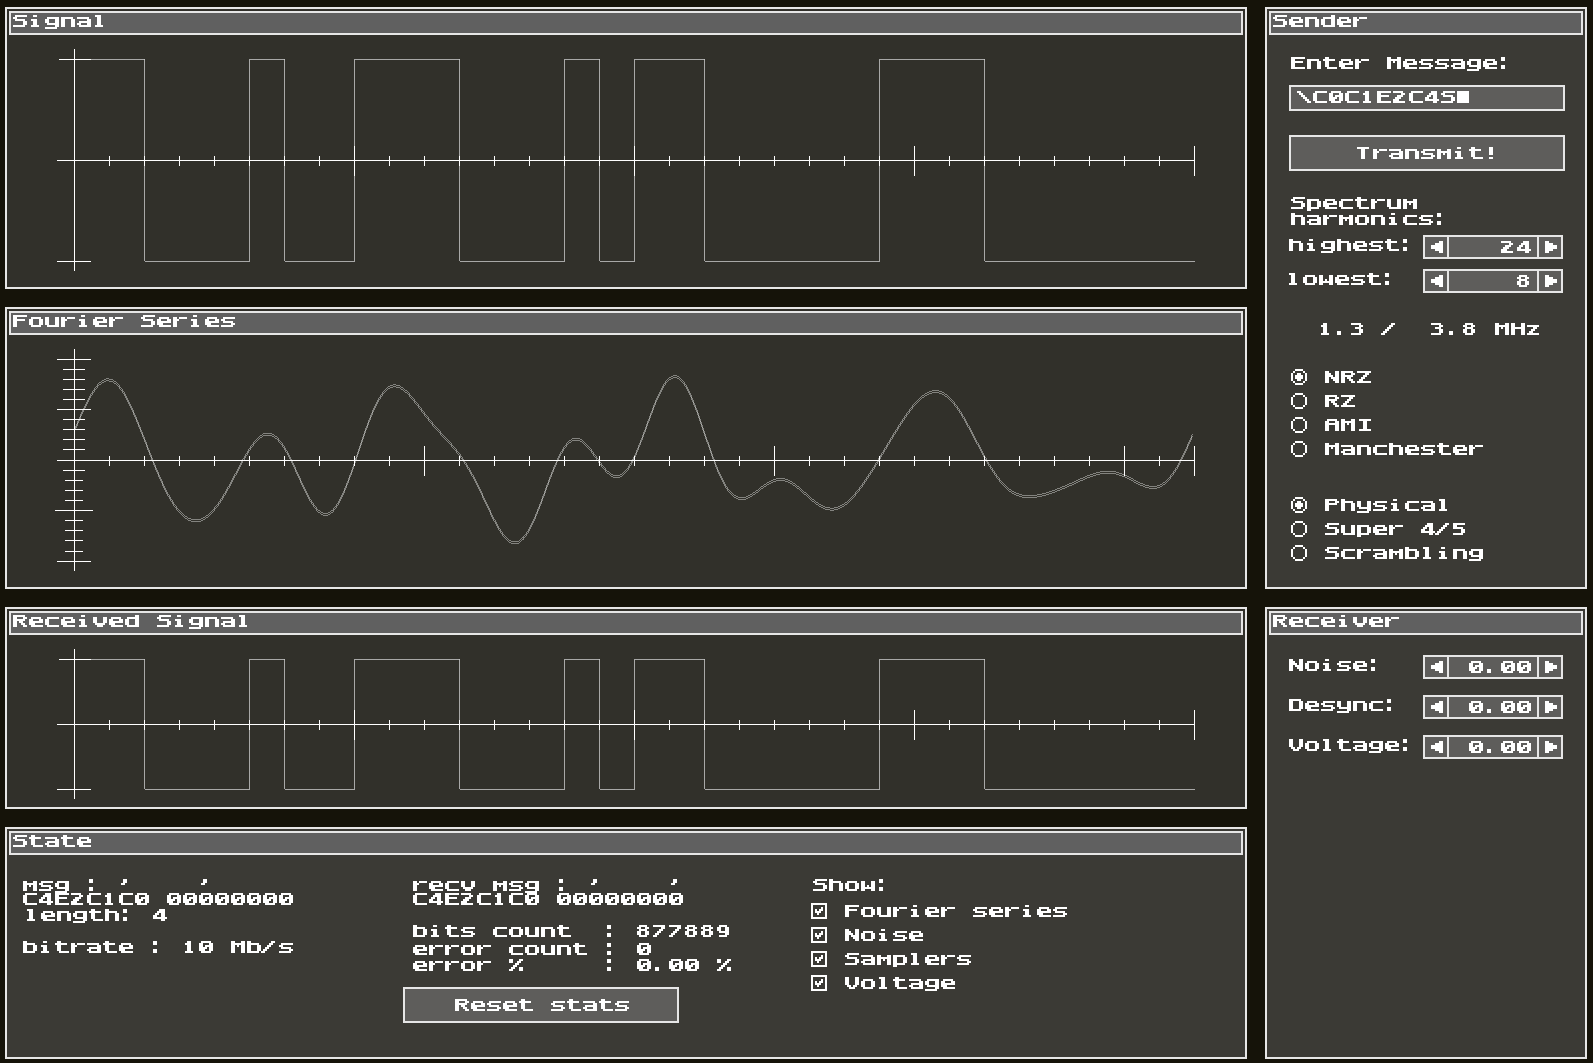
\includegraphics[width=0.95\linewidth]{./data/ideal_nrz_min_f.png}
	\caption{F = 1.3 - 3.8 Мгц}
\end{wrapfigure}

Для потенциальных методов кодирования, таких как NRZ или RZ, превалируют низкие частоты. При передаче конкретного сообщения нижняя частота всегда больше нуля и зависит от максимальной длины последовательностей нулей или единиц. В исходном сообщении, закодированном по методу NRZ, представленному на рисунке 1, низкочастотная составляющая образуется при передаче 6 последовательных нулей. Получается, что нижняя частота равна $\frac{C}{12}$, то есть при пропускной спобности $C = 10 \, \text{Мбит} / \text{с}$, указанной в программе, нижняя частота будет $\approx$ 0.83 Мгц. При этом верхняя граница частот будет образовываться при чередовании 0 и 1, что определяется из периода как $\frac{C}{2} = 5$ Мгц.

Проведя исследования, получили минимальную полосу пропускания идеального канала связи $F = 1.3 - 3.8 \, \text{Мгц}$. Спектр получился уже теоретического, в виду того, что это граничные значения, при которых вот-вот уже могут появиться ошибки. Для качественной предачи я бы значительно увеличил границу верхних частот, и уменьшил нижние частоты до рассчётных 0.8 Мгц.

\subsection{RZ}

\begin{wrapfigure}{r}{0.6\textwidth}
	\centering
	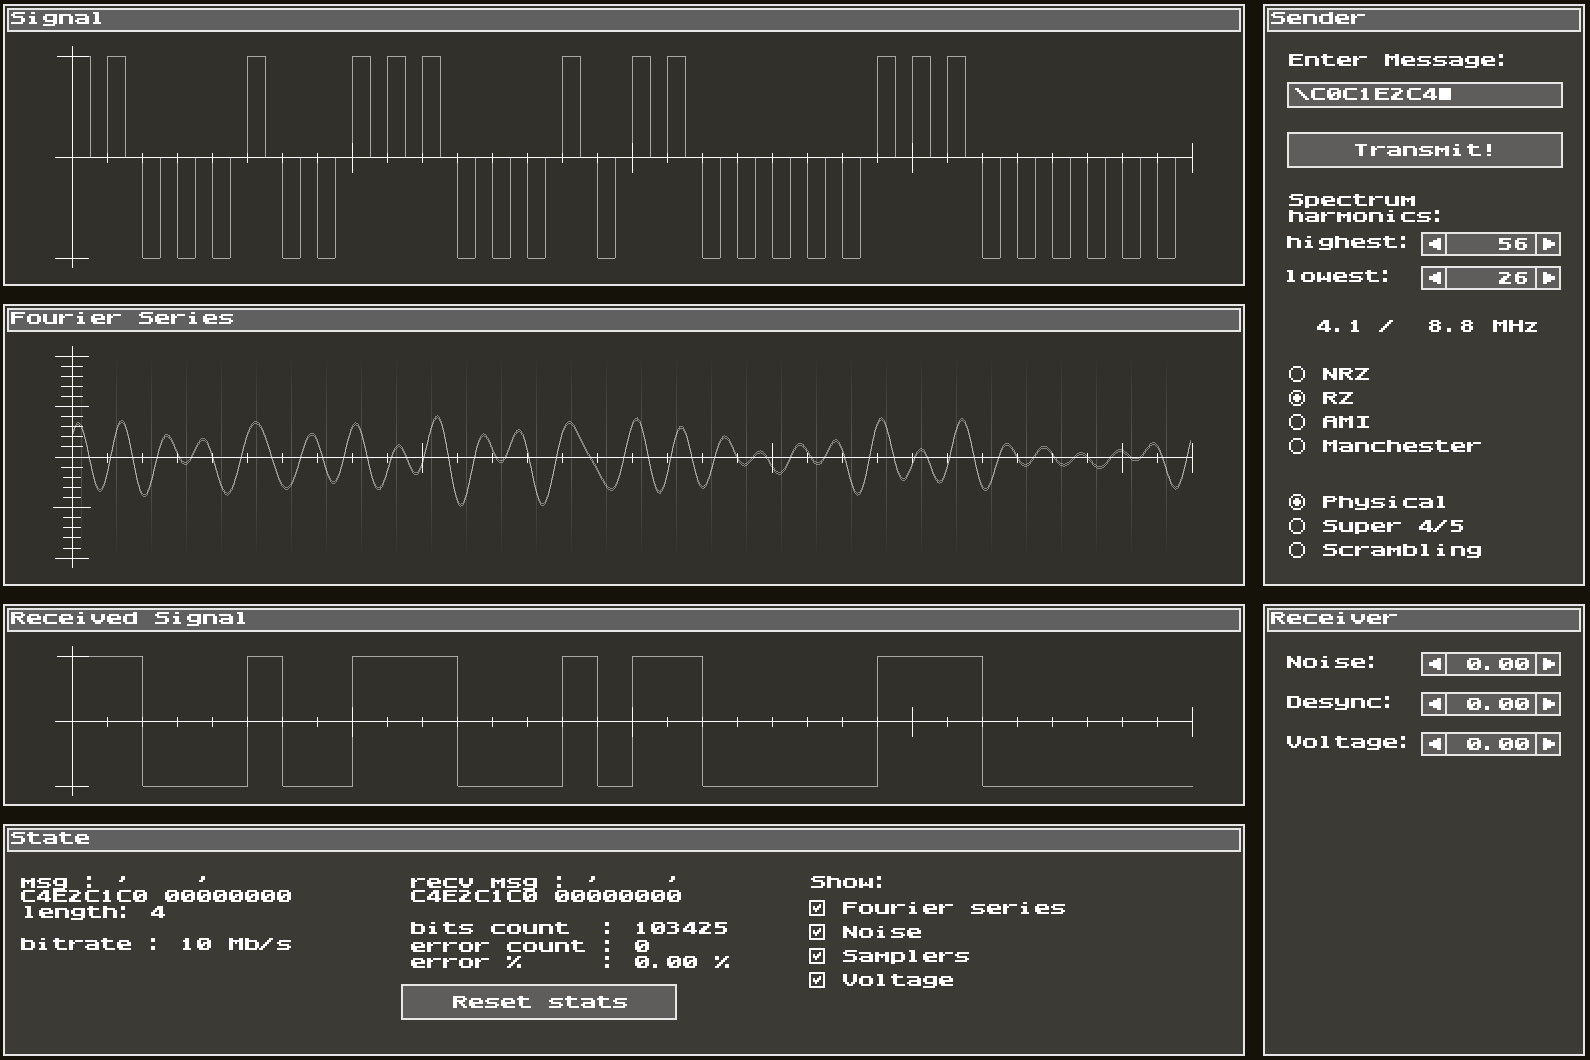
\includegraphics[width=0.95\linewidth]{./data/ideal_rz_min_f.png}
	\caption{F = 4.1 - 8.8 Мгц}
\end{wrapfigure}

Это тоже потенциальный метод кодирования, как и NRZ, поэтому низкочастотные особенности будут также иметь место и тут. В RZ верхняя частота достигается при передаче \textit{последовательных} значений 0 и 1, а нижняя - при передаче \textit{чередующихся} 0 и 1. период гармонического сигнала (синусоиды), используемого для передачи прямоугольных сигналов 0 и 1, будет равен длительности битового интервала $\tau$, умноженного на 5/2: $T = 2.5 \tau$. Тогда, нижняя граница частот $f_{\text{н}} = \frac{1}{T} = \frac{2C}{5}$, а верхняя $f_{\text{в}} = C$.


То есть, при пропускной способности канала связи $C = 10 \, \text{Мбит/с}$ частота основной гармоники равна $f_{\text{в}} = 10 \cdot 10^3 = 10 \, \text{МГц}$, битовый интервал $\tau = 100 \, \text{нс}$, $f_{\text{н}} = 4 \, \text{МГц}$. Следовательно, спектр: $S = f_{\text{в}} - f_{\text{н}} = 6 \, \text{МГц}$.

Проведя исследования, получили минимальную полосу пропускания идеального канала связи $F = 4.1 - 8.8 \, \text{Мгц}$, что уже теоретической в виду граничных, почти ошибочных значений. Для качественной предачи следует также значительно увеличить границу верхних частот, а нижние частоты практически совпали с рассчётными, что указывает на точность экспиримента.

\subsection{M2}

\begin{wrapfigure}{l}{0.58\textwidth}
	\centering
	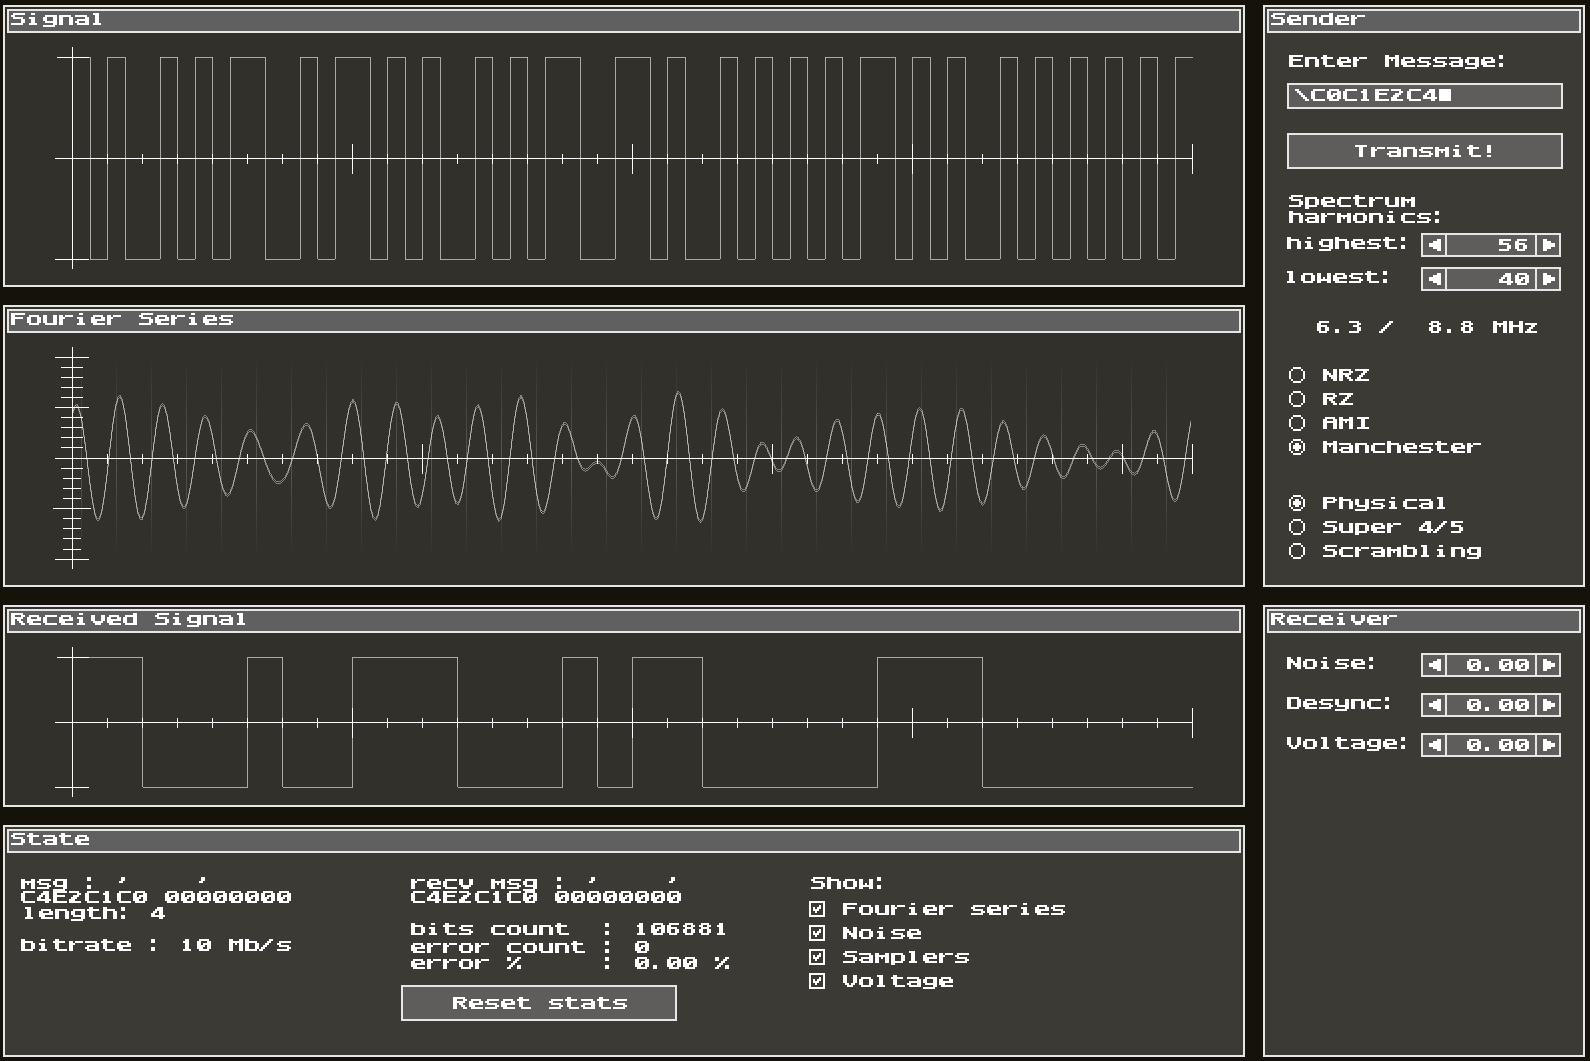
\includegraphics[width=0.95\linewidth]{./data/ideal_m2_min_f.png}
	% \cutpic{0.2cm}{9cm}{./data/ideal_m2_min_f.png}
	\caption{F = 6.3 - 8.8 Мгц}
\end{wrapfigure}

\vspace{-0mm}
Манчестерское кодирование - это импульсный метод кодирования. Это важное отличие от предыдущих методов, ведь кодирование сигнала импульсами позволяет избавиться от низкочастотных составляющих и соответственно их помех, а также улучшить синхронизацию.

Проведя аналогичные исследования, получили полосу в 2 раза уже теоретической, что демонстрирует повышенную устойчивость Манчестерского кодирования к помехам.

\subsection{Избыточное кодирование NRZ методом 4B/5B}

\newsavebox{\picbox}

Избыточное кодирование - это разновидность логического кодирования, применяемая в данном случае к потенциальному методу кодирования NRZ.

\begin{wrapfigure}{r}{0.6\textwidth}
	\centering
	\cutpic{0.2cm}{11cm}{./data/ideal_4b_5b.png}
	\caption{F =  2.0 - 4.5 Мгц}
\end{wrapfigure}


Суть избыточного кодирования - это улучшение синхронизации и устранение постоянной составляющей, которые присутствуют в моём сигнале при кодировании NRZ в виде последовательности повторяющихся значений <<0>> и/или <<1>>, с помощью замены каждых четырёх битов в исходном коде - пятью битами в результирующем, любое сочетание которых даёт 8 подряд расположенных <<1>> или 3 <<0>> в худшем случае.

Проведя исследования, получили минимальную полосу пропускания идеального канала связи $F = 2.0 - 4.5 \, \text{Мгц}$, что совпадает по ширине с минимальной полосой NRZ без избыточного кодирования, но отличается по диапазону частот - пришлось выполнять \textit{модуляцию} сигнала в более высокий диапазон частот.

\subsection{Скремблирование NRZ}

Сремблирование -  это также разновидность логического кодирования, суть которого заключается в применении определённого полинома к методу кодирования, в данном случае, NRZ, с целью уменьшения длинных последовательностей <<0>> и <<1>>.

\setlength{\intextsep}{0pt}
\setlength{\columnsep}{10pt}

\begin{wrapfigure}{r}{0.58\textwidth}
	\centering
	\cutpic{0.2cm}{11cm}{./data/ideal_nrz_scrambling.png}
	% 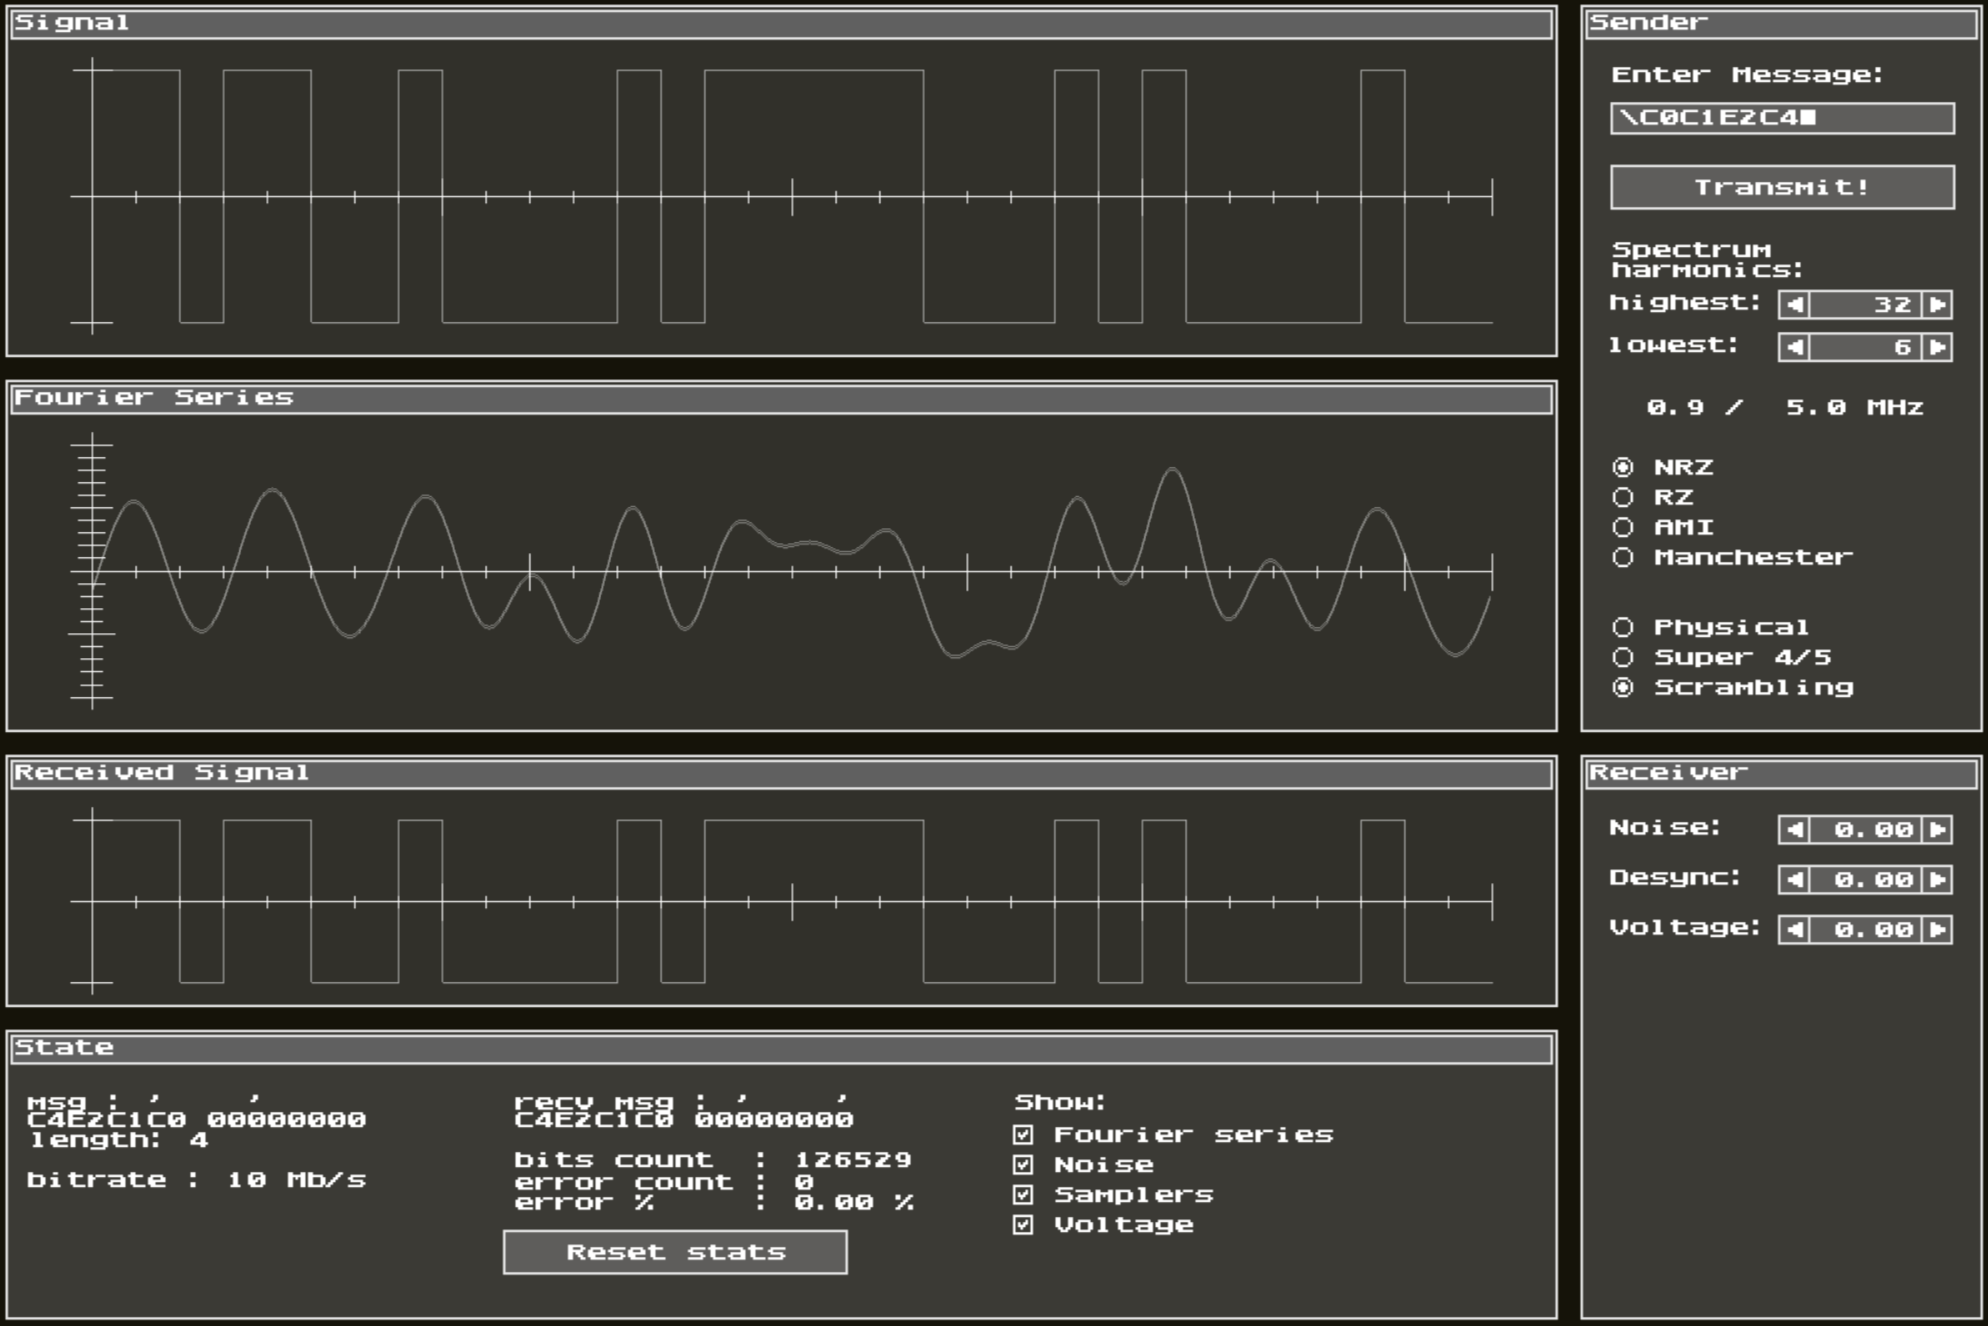
\includegraphics[width=0.95\linewidth]{./data/ideal_nrz_scrambling.png}
	\caption{F =  0.9 - 5.0 Мгц}
	\vspace{-140pt}
\end{wrapfigure}

Проведя исследования, получили минимальную полосу пропускания идеального канала связи $F = 0.9 - 5.0 \, \text{Мгц}$, то есть более широкую полосу пропускания, чем в базовом NRZ.
